\documentclass[dvipdfmx,a4paper]{jsarticle} % 日文 jsarticle 文类,A4 纸,dvipdfmx 驱动(适合日文+图像)
\usepackage{amsmath,amssymb,amsfonts,amsthm} % AMS 数学环境与符号(对齐公式、定理等)
\usepackage[dvipdfmx]{graphicx}              % 插图:\includegraphics
\usepackage{tikz}                            % TikZ 绘图
\usetikzlibrary{positioning, intersections, calc, arrows.meta, math, through, shadows,automata} % TikZ 扩展库
\usepackage{tcolorbox}                       % 彩色盒子环境(例题框、定理框等)
\tcbuselibrary{theorems,breakable}           % tcolorbox 的 “定理环境 + 可分页” 支持
\usepackage{enumerate}                       % 自定义编号列表,例如 \begin{enumerate}[(1)]
\usepackage{mathtools}                       % 对 amsmath 的扩展(:=号等)
\usepackage{caption}                        % 自定义公式标签样式
\usepackage{otf}                             % 和文 OTF 字体支持
\usepackage{xspace}                          % 自动在命令后加适当空格(给 \ie 之类命令用)
\usepackage{newpxtext}                       % Palatino 风格西文字体(正文)
\usepackage[utf8]{inputenc} %中国語コンパイル環境-cjkホットショット % 传统 pLaTeX 下的 UTF-8 输入编码
\usepackage{CJKutf8,CJKspace,CJKpunct} %中国語コンパイル環境 % CJK 中文/日文环境(配合 CJK 环境使用)
\usepackage{pgfplots}                        % 函数图、数据图绘制(基于 TikZ)
\usepackage{lastpage}                        % 获取最后一页页码(用来做 “Page x of y”)
\usepackage{fancyhdr}                        % 自定义页眉页脚
\pagestyle{fancy}                            % 使用 fancyhdr 作为默认页式
\fancyhf{}                                   % 清空默认页眉页脚
\fancyhead[L]{\textsc{情報科学Iの第十三回講義課題}} % 左页眉:课程/报告名称(自行修改)
\fancyhead[R]{\textit{www.andreyis.com}}    % 右页眉:网站/个人信息(自行修改)
\fancyfoot[C]{\thepage\quad \textit{of}\quad\pageref*{LastPage}} % 页脚中:Page x of y

\fancypagestyle{plain}{                      % 定义 plain 页式(章节首页等)
  \fancyhf{}                                 %   清空页眉页脚
  \renewcommand{\headrulewidth}{0pt}         %   去掉页眉横线
  \fancyfoot[C]{\thepage\quad \textit{of}\quad\pageref*{LastPage}} % 仍然保留页脚 Page x of y
}

\pgfplotsset{compat=1.18}                    % pgfplots 的版本兼容设置
\usepackage{okumacro} %漢字ruby              % 日文汉字 ruby(\ruby{漢字}{かんじ})

\renewcommand{\abstractname}{注意事項}       % 把 abstract 环境的标题 “Abstract” 改成 “注意事項”

\newtagform{textbf}[\textbf]{[}{]}           % 定义新的公式标签样式:加粗的 [1]
\usetagform{textbf}                          % 使用上面定义的标签样式

\newcommand*{\ie}{\textbf{\textit{i.e.}}\@\xspace} % 定义 \ie 命令(粗斜体 “i.e.”,自动空格)

\renewcommand{\qedsymbol}{$\blacksquare$}   % 证明结尾的 QED 符号改为黑方块 ■(amsthm 的 proof 环境用)

\newtcbtheorem[]{reidai}{例題}               % 定义 tcolorbox 风格的 “例題” 定理环境:\begin{reidai}{标题}{副标题}
{fonttitle=\gtfamily\sffamily\bfseries\upshape\large, % 标题字体:日文ゴシック+无衬线+粗体
 colframe=black,colback=black!15!white,     % 边框黑色,背景浅灰
 rightrule=1pt,leftrule=1pt,bottomrule=2pt, % 右/左/下边框线条粗细
 colbacktitle=black,theorem style=standard,breakable,arc=10pt} % 标题背景黑,正文可分页,圆角
{tha}                                       % 该定理环境的内部 name(用于交叉引用)

\renewcommand{\thefootnote}{\arabic{footnote}} % 脚注编号用阿拉伯数字

\newtheoremstyle{mystyle}%                  % 定义新的定理样式 mystyle
  {}%                      % 上部スペース (定理环境前的空白)
  {}%                      % 下部スペース (定理环境后的空白)
  {}%                      % 本文フォント (正文字体,默认)
  {}%                      % 1行目のインデント量 (标题行缩进)
  {\bfseries}%             % 見出しフォント (标题字体为粗体)
  :%                       % 見出し後の句読点 (标题后面的标点,这里是冒号)
  { }%                     % 見出し後のスペース (标题后与正文之间的空格)
  {\thmname{#1}\thmnumber{ #2}\thmnote{ (#3)}} % 标题格式:Thm 1 (备注)

\theoremstyle{mystyle}                       % 使用刚才定义的 mystyle 作为当前定理样式

% \setcounter{section}{0}                    % (示例)设置 section 计数器为 0(目前注释掉)
% \stepcounter{section}                      % (示例)把 section 计数器加一(目前注释掉)
% セクションカウンターを使用するが、表示はしない新しいセクションコマンドを作成 % 说明文字

\newtheorem{dfn}{\texttt{Def.}}[section]    % “定义”环境 dfn,标题显示为 “Def.”,按 section 编号
\newtheorem{exm}[dfn]{\texttt{Ex.}}         % “例子”环境 exm,与 dfn 共用同一个编号
\newtheorem{prop}[dfn]{\texttt{Prop.}}      % 命题环境 prop
\newtheorem{lem}[dfn]{\texttt{Lem.}}        % 引理环境 lem
\newtheorem{thm}[dfn]{\texttt{Thm.}}        % 定理环境 thm
\newtheorem{cor}[dfn]{\texttt{Cor.}}        % 推论环境 cor
\newtheorem{rem}[dfn]{\texttt{Rem.}}        % 备注环境 rem
\newtheorem{fact}[dfn]{\texttt{Fact}}       % 事实环境 fact

\renewcommand{\qedsymbol}{$\blacksquare$}   % 再次确认 QED 符号为黑方块(如果前面被别的包改掉)

\usepackage{lipsum} % 用于生成示例文本(\lipsum[1-2] 生成假文)
\usepackage{float} % 强制浮动(使用 [H] 选项固定图表位置)
\usepackage{tikz} % 用于定位(重复引入 TikZ,其实可以和前面的合并)

% 排版相关的自定义命令:印 “解答 / 証明 / 補足 / 注意” 标签的小盒子

\newcommand{\kai}% 解答框标题:“解答”
{\noindent
\begin{tikzpicture}[scale=0.2, baseline=2.8pt]
\draw (3.3,1.2) node{\large\textgt{解 答}}; % 文字“解答”
\draw[thick, rounded corners=3pt,] (0,0)--(6.5,0)--(6.5,2.4)--(0,2.4)--cycle; % 带圆角的矩形外框
\end{tikzpicture}} % 使用方式:写在解答前一行,\kai

\newcommand{\shomei}% 証明框标题:“証明”
{\noindent
\begin{tikzpicture}[scale=0.2, baseline=2.8pt]
\draw (3.3,1.2) node{\textgt{証 明}}; % 文字“証明”
\draw[double,thick,rounded corners=3pt,] (0,0)--(6.5,0)--(6.5,2.4)--(0,2.4)--cycle; % 双线矩形外框
\end{tikzpicture};} % 使用方式:写在证明前一行,\shomei

% 補足框
\newcommand{\hosoku}{\noindent
\begin{tikzpicture}[scale=0.2, baseline=2.8pt]
\draw (6,1) node{\large\textgt{補足}}; % 文字“補足”
% 左侧小菱形装饰
\fill (0,1)--(1,0)--(2,1)--(1,2)--cycle;
\fill[gray] (1,1)--(2,0)--(3,1)--(2,2)--cycle;
\fill (2,1)--(3,0)--(4,1)--(3,2)--cycle;
% 右侧小菱形装饰
\fill (10,1)--(11,0)--(12,1)--(11,2)--cycle;
\fill[gray] (9,1)--(10,0)--(11,1)--(10,2)--cycle;
\fill (8,1)--(9,0)--(10,1)--(9,2)--cycle;
\end{tikzpicture};} % 使用方式:\hosoku 后面接补充说明文字

% 注意框
\newcommand{\chui}{\noindent
\begin{tikzpicture}[scale=0.2, baseline=2.8pt]
\fill (0,0)--(6.5,0)--(6.5,2.2)--(0,2.2); % 填满背景色(默认黑)
\draw (3.3,1) node[white]{\large\textgt{注意!}}; % 中间白字“注意!”
\draw[thick] (0,0)--(6.5,0)--(6.5,2.2)--(0,2.2)--cycle; % 外框
\end{tikzpicture};} % 使用方式:\chui 后面写注意内容

% 标题信息:可以根据实际报告修改 title / author / date

\title{\vspace{-3cm} 情報科学Iの第十三回講義課題}  % 标题:目前设置为“空”,仅挤掉竖直空间(可改成真正的标题)
\author{\texttt{YI Ran} - $\mathnormal{21122200512}$\\ \texttt{andreyi@outlook.jp}}  % 作者:姓名+学号+邮箱
\date{\today}  % 日期:自动使用当天日期

\begin{document}
\maketitle                                   % 输出标题页
\thispagestyle{plain}                        % 这一页使用 plain 样式(我们前面定义过)

% 下方是可选的 QR 码 + 文字示例,目前全部注释掉
% \vspace{-0.4cm}
% \begin{figure}[H]
% \centering
% \begin{tikzpicture}[remember picture, overlay]
%    \node[anchor=north east] at (current page.north east) {%
%         \includegraphics[width=2cm]{pics/qr.png} % 这里改成你真正的 QR 图片路径
%     };
%     \node[anchor=north east, yshift=-2cm] at (current page.north east) {デジタル版はここ};
% \end{tikzpicture}
% \label{fig:my_label}
% \end{figure}

% \begin{abstract} %概要
  % 注意事項:如果需要写“注意事项”,可取消注释此 abstract 环境
% \end{abstract}

% 例題环境示例(使用 \begin{reidai}{主标题}{副标题})
% \begin{reidai}{2次方程式}{解答}
% ここに例題の内容を書く。
% \end{reidai}
% \begin{proof}
% ここに証明を書く。
% \end{proof}

%ーーーーー問1------
\section*{\textbf{問1}\quad \normalfont\Large 図1のオートマトン$M_1$について答えよ} % 第一节标题(可以直接改文字)
\textbf{(1)}\quad $M_1$が受理する記号列を3つあげよ。\\
\indent
\textbf{(2)}\quad $M_1$が却下する記号列を3つあげよ。\\
\indent
\textbf{(3)}\quad $M_1$の言語$L(M_1)$はどのような集合か?\\

\begin{figure}[htbp]
\raggedright
\begin{minipage}{\linewidth}
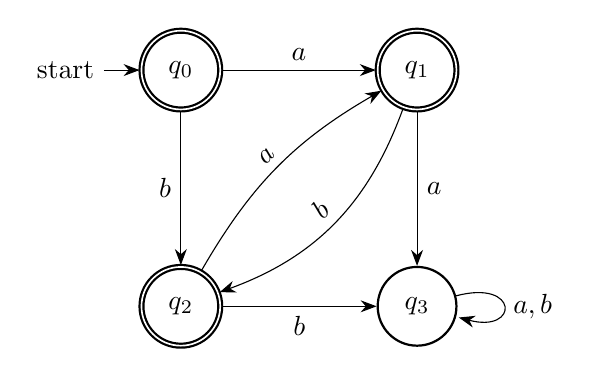
\begin{tikzpicture}[
    >={Stealth[scale=1.2]},
    node distance=3cm,
    on grid,
    auto,
    every state/.style={thick, minimum size=1cm}
]

% 定义状态节点
\node[state, initial, accepting] (q0) {$q_0$};
\node[state, accepting, right=of q0] (q1) {$q_1$};
\node[state, accepting, below=of q0] (q2) {$q_2$};
\node[state, below=of q1] (q3) {$q_3$};

% 定义转移
\path[->]
    (q0) edge node {$a$} (q1)
    (q0) edge node[swap] {$b$} (q2)
    (q1) edge node {$a$} (q3)
    (q2) edge[bend left=15]  node[sloped, above] {$a$} (q1) % q2 -> q1
    (q1) edge[bend left=25]  node[sloped, above] {$b$} (q2) % q1 -> q2
    (q2) edge node[swap] {$b$} (q3)
    (q3) edge[loop right] node {$a,b$} (q3);

\end{tikzpicture}
\vspace{1em}
\captionsetup{justification=raggedright, singlelinecheck=false,margin={4em,0pt}}
\caption{決定性オートマトン $M_1$}
\label{fig:dfa_m1}
\end{minipage}
\end{figure}
\kai\\

\indent
\textbf{(1)}\quad aba,\ bab,\ abab\\
\indent
\textbf{(2)}\quad aa,\ bba,\ aab\\
\indent
\textbf{(3)}\quad $L(M_1)$は、連続する重複文字を持たない文字列の集合である。\\
\indent
\quad\quad\ie $L(M_1) = (ab)^{\star}(\varepsilon \cup a) \cup (ba)^{\star}(\varepsilon \cup b) = (\varepsilon \cup b)(ab)^{\star}(\varepsilon \cup a)$
\newpage
%ーーーーー問2------
\section*{\textbf{問2}\quad \normalfont\Large 図2のオートマトン$M_2$について答えよ}
\textbf{(1)}\quad 次の入力列のうち、$M_2$によって受理されるものをすべて選べ。\\
\indent
\quad \quad aa, aaa, aaaa, ababa, babab, $ \mathrm{\varepsilon} $\\
\indent
\textbf{(2)}\quad $M_2$の言語$L(M_2)$はどのような集合か?\\

\begin{figure}[htbp]
\raggedright
\begin{minipage}{\linewidth}
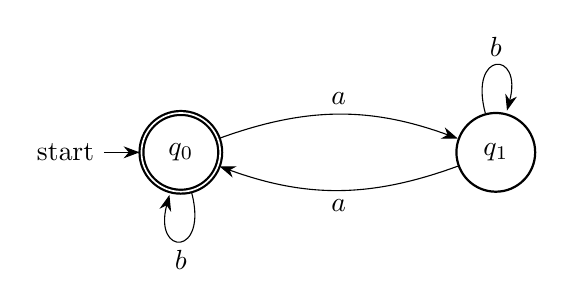
\begin{tikzpicture}[
    >={Stealth[scale=1.2]},
    node distance=4cm,
    on grid,
    auto,
    every state/.style={thick, minimum size=1cm}
]

% 状态节点
\node[state, initial, accepting] (q0) {$q_0$};
\node[state, right=of q0] (q1) {$q_1$};

% 状态自环
\path[->] (q0) edge[loop below] node {$b$} (q0);
\path[->] (q1) edge[loop above] node {$b$} (q1);

% 状态间转移
\path[->] (q0) edge[bend left=20] node[above] {$a$} (q1);
\path[->] (q1) edge[bend left=20] node[below] {$a$} (q0);

\end{tikzpicture}

\vspace{1em}
\captionsetup{justification=raggedright, singlelinecheck=false,margin={4em,0pt}}
\caption{決定性オートマトン $M_2$}
\label{fig:dfa_example}
\end{minipage}
\end{figure}

\kai\\

\indent
\textbf{(1)}\quad aa,\ aaaa,\ babab,\ $ \mathrm{\varepsilon} $\\
\indent
\textbf{(2)}\quad $L(M_2)$は、文字 $a$ の出現回数が偶数であるような文字列の集合である。\\
\indent
\quad\quad\ie $L(M_2) = (b\cup b^{\star}ab^{\star}a)^{\star}$

%ーーーーー問3------
\section*{\textbf{問3}\quad \normalfont\Large 図3のオートマトン$M_3$について答えよ}
\textbf{(1)}\quad $M_3$が受理する記号列を3つあげよ。\\
\indent
\textbf{(2)}\quad $M_3$の言語$L(M_3)$はどのような集合か?\\

\begin{figure}[htbp]
\raggedright
\begin{minipage}{\linewidth}
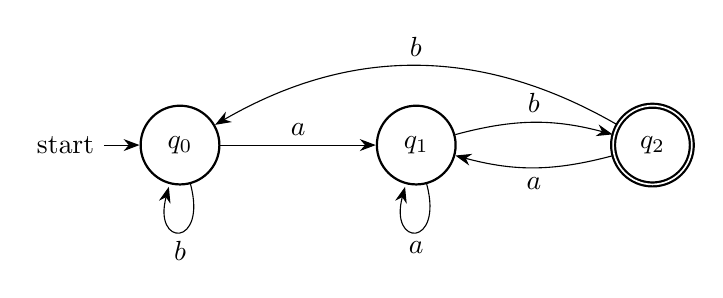
\begin{tikzpicture}[
    >={Stealth[scale=1.2]},
    node distance=3cm,
    on grid,
    auto,
    every state/.style={thick, minimum size=1cm}
]

% 状态节点
\node[state, initial] (q0) {$q_0$};
\node[state, right=of q0] (q1) {$q_1$};
\node[state, accepting, right=of q1] (q2) {$q_2$};

% 自环
\path[->] (q0) edge[loop below] node {$b$} (q0);
\path[->] (q1) edge[loop below] node {$a$} (q1);

% 状态间转移
\path[->] (q0) edge node {$a$} (q1);
\path[->] (q2) edge[bend right=30] node[above] {$b$} (q0);
\path[->] (q1) edge[bend left=15] node[above] {$b$} (q2);
\path[->] (q2) edge[bend left=15] node[below] {$a$} (q1);

\end{tikzpicture}

\vspace{1em}
\captionsetup{justification=raggedright, singlelinecheck=false, margin={4em,0pt}}
\caption{決定性オートマトン $M_3$}
\label{fig:dfa_three_states}
\end{minipage}
\end{figure}

\kai\\
\indent
\textbf{(1)}\quad $ab$,\ $aab$,\ $babab$ \\
\indent
\textbf{(2)}\quad $L(M_3)$は、文字 $a$, $b$ からなる文字列のうち、末尾が $ab$ であるものの集合である。\\
\indent
\quad\quad\ie $L(M_3) = (a\cup b)^{\star}ab$

%ーーーーー問4------
\section*{\textbf{問4}\quad \normalfont\Large 図4のオートマトン$M_4$について答えよ}
\textbf{(1)}\quad 次の入力列のうち、$M_4$によって受理されるものをすべて選べ。\\
\quad\quad\quad abc, cba, $\mathrm{\varepsilon}$, a, b, abcab, aabbcc\\
\indent
\textbf{(2)}\quad $M_4$の言語$L(M_4)$はどのような集合か?\\

\begin{figure}[htbp]
\raggedright
\begin{minipage}{\linewidth}
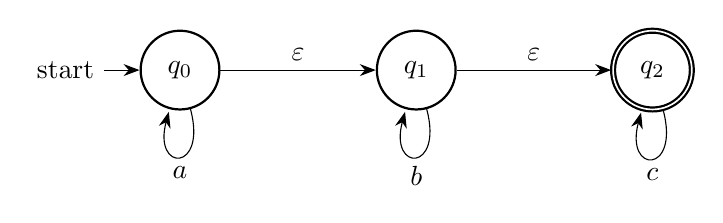
\begin{tikzpicture}[
    >={Stealth[scale=1.2]},
    node distance=3cm,
    on grid,
    auto,
    every state/.style={thick, minimum size=1cm}
]

% 状态节点
\node[state, initial] (q0) {$q_0$};
\node[state, right=of q0] (q1) {$q_1$};
\node[state, accepting, right=of q1] (q2) {$q_2$};

% 自环
\path[->] (q0) edge[loop below] node {$a$} (q0);
\path[->] (q1) edge[loop below] node {$b$} (q1);
\path[->] (q2) edge[loop below] node {$c$} (q2);

% ε转移
\path[->] (q0) edge node {$\varepsilon$} (q1);
\path[->] (q1) edge node {$\varepsilon$} (q2);

\end{tikzpicture}

\vspace{1em}
\captionsetup{justification=raggedright, singlelinecheck=false, margin={4em,0pt}}
\caption{非決定性オートマトン $M_4$}
\label{fig:nfa_epsilon}
\end{minipage}
\end{figure}

\kai\\

\indent
\textbf{(1)}\quad abc,\ $\varepsilon$,\ a,\ b,\ aabbcc\\
\indent
\textbf{(2)}\quad $L(M_4)$は、0個以上の a の後に 0個以上の b が続き、その後に 0個以上の c が続く文字列の集合である。\ie $L(M_4) = a^{\star}b^{\star}c^{\star}$
\end{document}